\documentclass{report}
\usepackage{graphicx} % Required for \includegraphics
\usepackage{float}    % Required for [H] specifier

\begin{document}
\title{Labwork 4: Report}
\author{Nguyen Nhat Anh} % Required by the report class for \maketitle
\maketitle

\section{Introduction}
I have made the image RGB-to-gray converter using Numba CUDA, implementing to 2D arrays. All the code given are following strictly from report. 

\section{Results}
For CPU:
\begin{figure}[H]
    \centering 
    \includegraphics[width=0.7\linewidth]{cpu_output.jpg}
    \caption{CPU image output.}
    \label{fig:cpu_image} 
\end{figure}

For GPU:
\begin{figure}[H]
    \centering 
    \includegraphics[width=0.7\linewidth]{output_gpu.jpg}
    \caption{GPU image output.}
    \label{fig:gpu_image}
\end{figure}

Performance comparison:
\begin{figure}[H]
    \centering 
    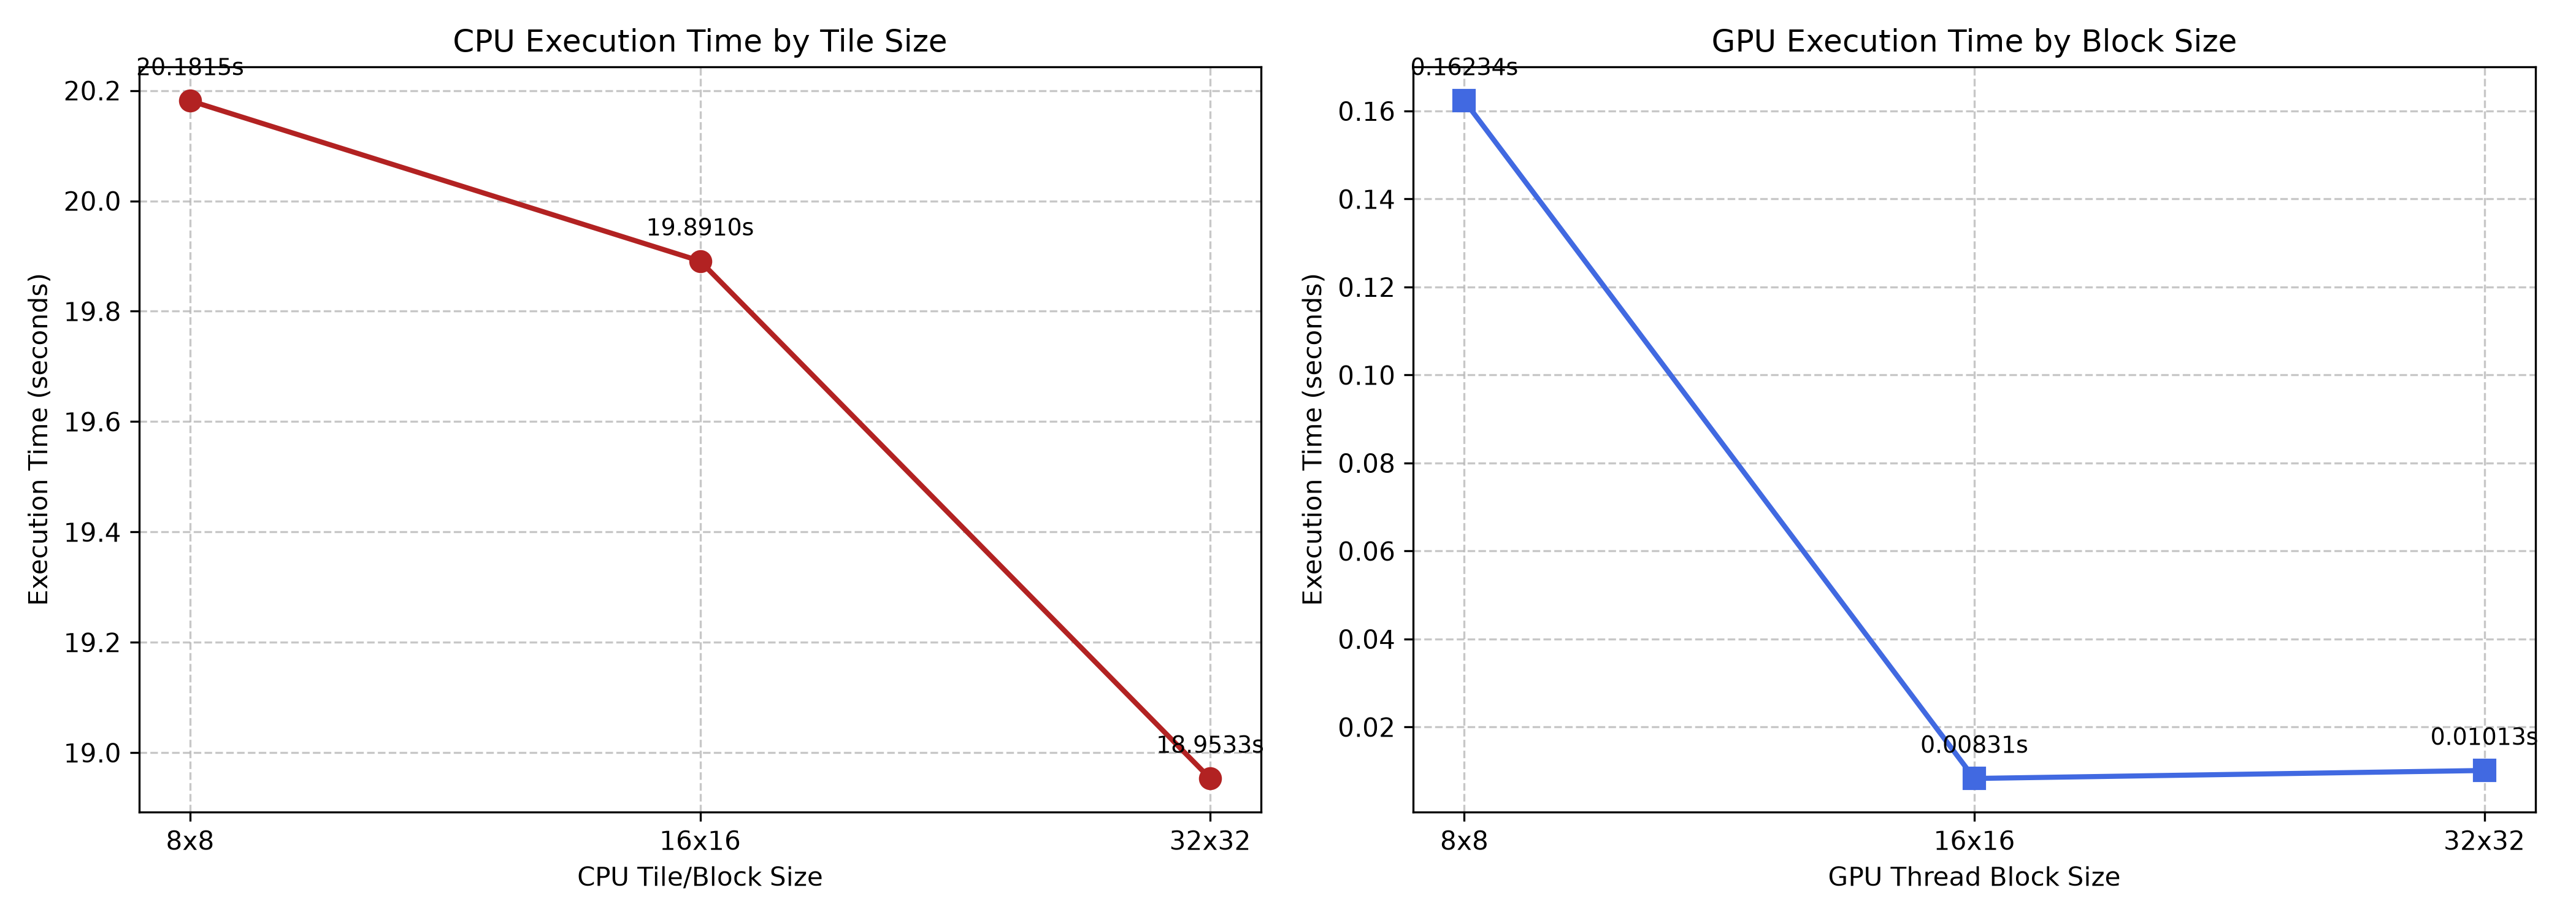
\includegraphics[width=0.7\linewidth]{per.png}
    \caption{Performance comparison between CPU and GPU.}
    \label{fig:performance_image}
\end{figure}

Runtime comparison:
\begin{figure}[H]
    \centering 
    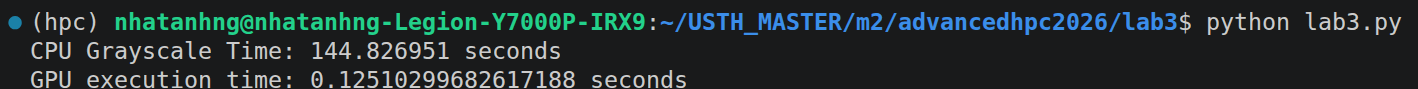
\includegraphics[width=0.7\linewidth]{runtime.png}
    \caption{Runtime comparison between CPU and GPU for 1D array (Block Size 64).}
    \label{fig:runtime_image}
\end{figure}


\begin{figure}[H]
    \centering 
    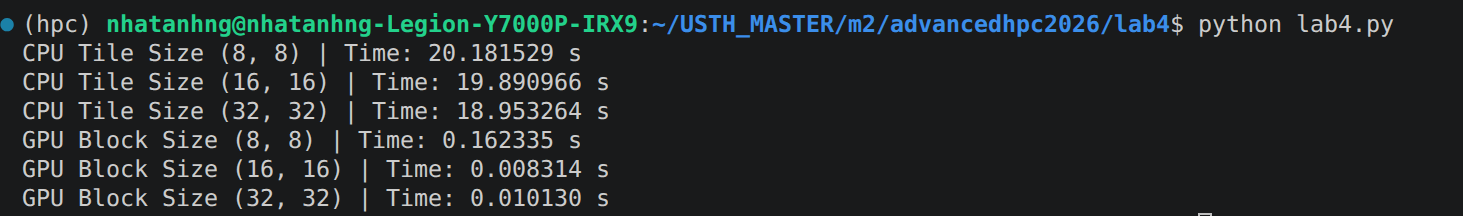
\includegraphics[width=0.7\linewidth]{runtime_2.png}
    \caption{Runtime comparison between CPU and GPU for 2D array.}
    \label{fig:runtime_2_image}
\end{figure}

\section{Discussion}
The results show that, for the CPU, the higher the block size, the better the performance, 
while for the GPU, the best one is for block size 16x16. Compared to the running in 1D array, with respect to block size 64, 
the performance of the CPU is improved significantly, but the performance of the GPU is slightly worse.
In overall, the GPU implementation significantly outperforms the CPU implementation in terms of runtime.
\end{document}